\documentclass[]{rAMF2e}
%\usepackage[square]{natbib}
%\usepackage{authblk}
\usepackage{listings}
\usepackage[center]{caption}


\begin{document}
\doi{}
\issn{}  \issnp{}
\jvol{00} \jnum{00} \jyear{2013} %\jmonth{January--March}
\def\jobtag{}
\publisher{Unpublished}
\jname{}

\markboth{Fabien {Le Floc'h}, Gary Kennedy}{Draft}

\title{Finite Difference Techniques for Arbitrage Free SABR}
\author{Fabien {Le Floc'h}$^\star$\thanks{{\em{Correspondence Address}}: Calypso Technology, 106 rue de La Bo\'{e}tie, 75008 Paris. Email: \texttt{fabien\_lefloch@calypso.com} \vspace{6pt}} and Gary Kennedy$^\dag$}
\affil{$^\star$Calypso Technology, 106 rue de La Bo\'{e}tie, 75008 Paris\\$^\dag$Clarus Financial Technology, London}
%
\date{\today}
\received{v1.1 released June 2013}

\maketitle
\newcommand{\sgn}{\mathop{\mathrm{sgn}}}
\begin{abstract}
This paper presents various finite difference schemes applied to the SABR arbitrage free density problem with a focus on stability and speed.
\begin{keywords}stochastic volatility, SABR, TR-BDF2, Crank-Nicolson, finite difference, finance\end{keywords}
\end{abstract}

\section{Introduction}
It is now well known that original SABR analytic formula from \citep{hagan2002managing} used to compute options implied volatilities is not arbitrage free. Especially, the probability density can become negative for low strikes and long maturities. Given the low rates environment we live in today, many authors have proposed various improvements to the original formula \citep{obloj2007fine, johnson2009arbitrage, paulot2009asymptotic, benaim2008arbitrage}.  A single step finite difference method is proposed in \citep{andreasen2011zabr} which leads to an arbitrage free SABR-like model. While the approach from Andreasen and Huge converges for short maturities to the original SABR analytic formula, it is deliberately different, even at the money, for longer expiries.


Hagan himself proposed a new arbitrage free SABR solution, based on a finite difference discretization of the probability density in \citep{hagan2013arbitrage}. This approach allows to stay very close to the original SABR analytic formula, well known and widely used, while being arbitrage free, and thus allows pricing with low rates. The authors use a Crank-Nicolson time-stepping, which is known to have oscillation issues \citep{GiCa2006} as it is only $A$-stable but not $L$-stable \citep{Le07}. We will show that this issue arises in the context of SABR pricing, and propose alternative schemes with increased stability. Speed and accuracy were key ingredients in popularising the original SABR formula. Given that for a 30 year cap on a 3M LIBOR, there are potentially 119 PDE to solve, we will focus our attention to performance of the proposed schemes, as well as to what extent the discretization grid can be reduced in size.

\section{Arbitrage Free SABR}
In \citep{hagan2013arbitrage}, pricing in SABR with parameters $\alpha, \beta, \rho, \nu$ and forward $f$ at $T$ relies on the solution of a PDE on the probability density $Q$:

\begin{align}\label{eqn_pde}
\frac{\partial Q}{\partial T}(T,F) = \frac{\partial^2 M(T,F) Q(T,F)}{\partial F^2} \text{ and } \begin{cases}
\frac{\partial Q_L}{\partial T}(T) = \lim_{F \to F_{min}} \frac{\partial M(T,F) Q(T,F)}{\partial F}\\
\frac{\partial Q_R}{\partial T}(T) = \lim_{F \to F_{max}} \frac{\partial M(T,F) Q(T,F)}{\partial F}
\end{cases}
\end{align}
with
\begin{alignat}{2}
M(T,F) &= \frac{1}{2} \alpha^2 (1+2\rho\nu z+ \nu^2 z^2) e^{\rho\nu\alpha\Gamma T} C^2(F) &\text{, }
\Gamma(F) &= \frac{C(F)-C(f)}{F-f}\\
z(F) &= \frac{1}{\alpha (1-\beta)}(F^{1-\beta}-f^{1-\beta}) &\text{, }
C(F) &= F^{\beta} 
\end{alignat}

It is suggested that the lower boundary $F_{min}$ for the standard SABR model is at zero. As the finite difference grid described in Appendix C of their paper starts at  $F_0 = F_{min} - \frac{h}{2}$ where $h$ is the asset forward discretization step size, this implies the evaluation of various quantities with a negative forward $F_0$, while some of those quantities are undefined for negative forwards. Fortunately, only the product $M_0 Q_0$ is used in the discretization of equation (\ref{eqn_pde}) and it is entirely defined by $M_1 Q_1$  because of the mirror-like boundary condition (imposed at the fictitious point $F_0$): 
\begin{align}\label{boundary_condition}
M_0 Q_0 + M_1 Q_1 &= 0
\end{align}
As long as $M_0 \neq 0$, $M_0 Q_0$ will take the value $-M_1 Q_1$. For example, we can use $|F_0|$ to compute $M_0$ and this will result in a symmetry around $F_{min}$.


Another alternative would be to place the grid so that $F_0 = F_{min}$ and use boundary condition $Q_0 = 0$ there. The probability of absorption $Q_L$ could then be evaluated using an forward finite difference first derivative estimate. This would result in the exact same equation as (C.10a) of their paper and the scheme would still be moment preserving. However this comes at a cost of a slight loss of accuracy as, effectively, the derivative will be estimated using $Q_1 = Q(h)$ instead of $Q_1 = Q(\frac{h}{2})$.

The formula for $\Gamma$ is also undefined for $F=f$, in which case we just use $\Gamma(f) = \frac{\partial C}{\partial F}(f)$.

\section{Crank-Nicolson Oscillations with SABR}\label{section_cn}
\begin{figure}[htb]
  \begin{center}  
    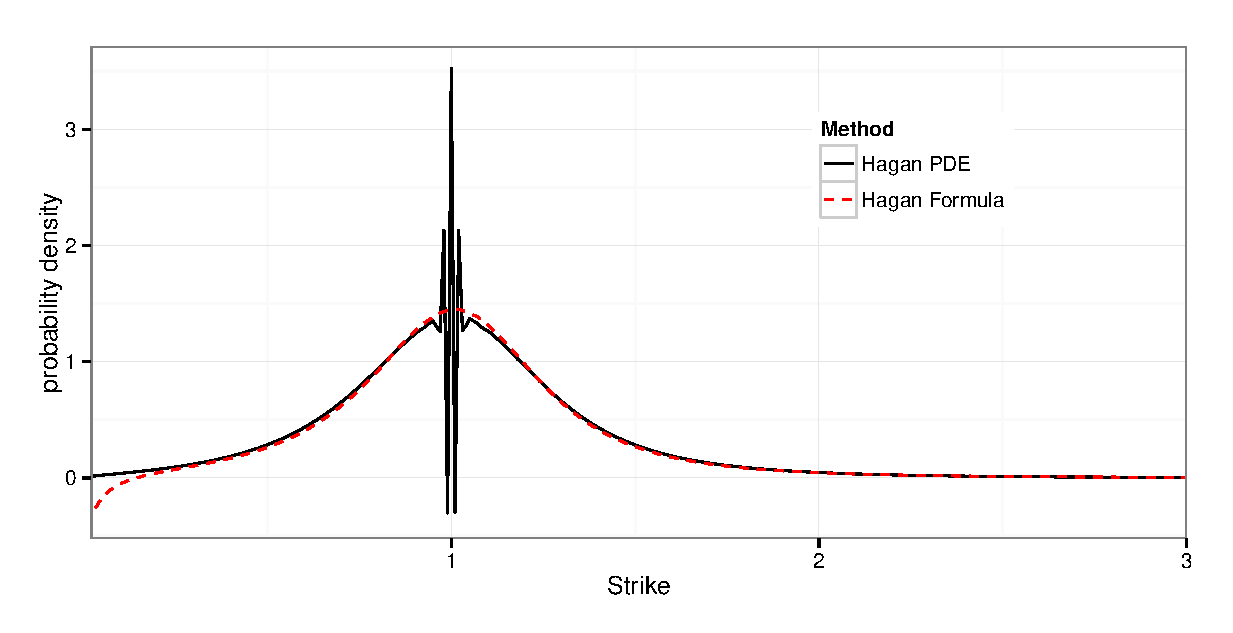
\includegraphics[width=12cm]{density_hagan_cn_500_40.eps}
  \end{center}
     \caption{\label{fig:density_hagan_cn_500_40} Probability density in Hagan PDE discretized with Crank-Nicolson with 500 points and 40 time-steps. $\alpha=35\%, \beta=0.25, \rho=-10\%, \nu=100\%, T=1$}
\end{figure}

We use the same parameters as the example of negative density with the standard SABR formula in \citep{hagan2013arbitrage}: $\alpha=35\%, \beta=0.25, \rho=-10\%, \nu=100\%$ and forward $f=1$ at $T=1$, a relatively fine discretization in the rate dimension (500 points, that is $h = 0.01005$) and large time-steps (40 steps, that is $\delta=0.025$). \cite{hagan2013arbitrage} recommend between 200 and 500 points and 30 to 100 time-steps.

Figure \ref{fig:density_hagan_cn_500_40} shows strong oscillations around the forward. To guarantee the absence of oscillations, the \emph{Courant number}  should be small enough $\Psi = M \frac{\delta}{h^2}\leq 1$. This corresponds directly to the stability of the explicit Euler part of Crank-Nicolson. In practice, a higher value is acceptable because of a slight damping in Crank-Nicolson \citep{lawson1978extrapolation}. $M$ depends on $F$, but we can use the at-the-money value at $f$, as the spike is located at-the-money, that is 
\begin{align}
\Psi &= \frac{1}{2} \alpha^2 (1+2\rho\nu z+ \nu^2 z^2) e^{\rho\nu\alpha\beta f^{\beta-1} T} f^{2\beta} \frac{\delta}{h^2}
\end{align} 

\begin{figure}[htb]
  \begin{center}  
    \subfigure[with 40 time steps]{\label{fig:density_hagan_cn_500_40_5}
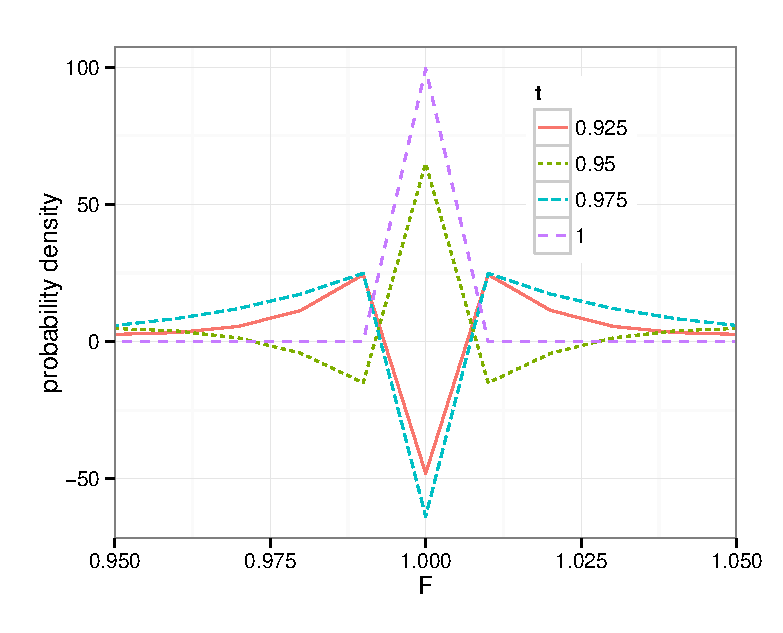
\includegraphics[width=7cm]{density_hagan_cn_500_40_5.eps}}
  \subfigure[with 1280 time steps]{\label{fig:density_hagan_cn_500_1280_5}
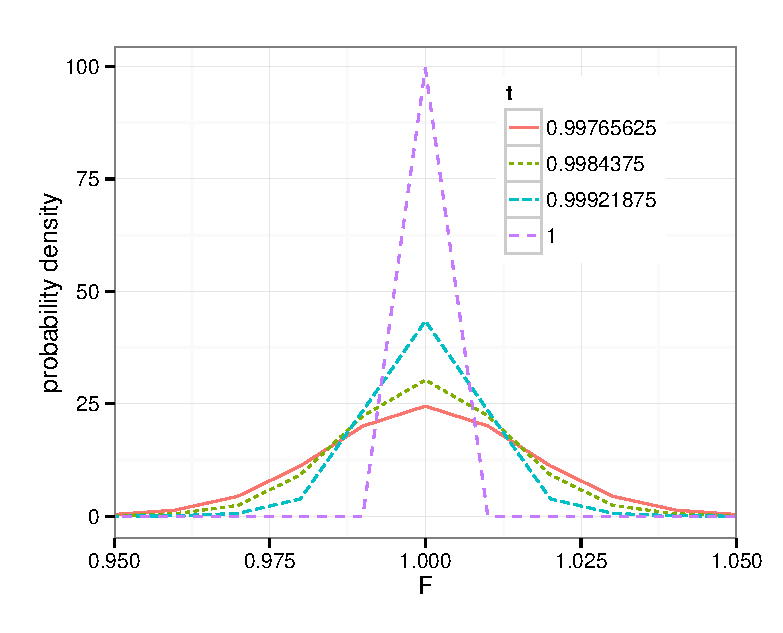
\includegraphics[width=7cm]{density_hagan_cn_500_1280_5.eps}}
  \end{center}
     \caption{\label{fig:density_hagan_500_40_5} First 4 time steps of the probability density in Hagan PDE discretized with Crank-Nicolson}
\end{figure}

In our example, in Figures \ref{fig:density_hagan_cn_500_40} and \ref{fig:density_hagan_cn_500_40_5} $\Psi \approx 15$ while Figure \ref{fig:density_hagan_cn_500_1280_5} shows that in deed when $\Psi < 1$ there are no oscillations. We will see in the next sections that a much smaller number of time steps can be used, while still preserving good accuracy, with other finite difference time-stepping techniques.

\section{Alternative Schemes}
The boundary condition described by equation (\ref{boundary_condition}) is applicable to all schemes considered in this section as it is independent of the time-stepping.

\subsection{Rannacher}
A common fix for Crank-Nicolson oscillations related to non smooth initial data is Rannacher time-stepping \citep{rannacher1984finite, GiCa2006}. It consists in introducing two half time-steps of implicit Euler time-stepping before applying Crank-Nicolson, because implicit Euler has much stronger damping properties. This comes at a cost in accuracy as implicit Euler is an order-1 scheme in time, especially when only a few time-steps are needed. 
The SABR density discretization will still be moment preserving if we discretize the Euler half steps as:
\begin{align}\label{eqn_euler_1}
Q_j^{n+\frac{1}{2}}-Q_j^n &= \frac{\delta}{2h^2} \left(M_{j+1}^{n+\frac{1}{2}}Q_{j+1}^{n+\frac{1}{2}}-2M_j^{n+\frac{1}{2}}Q_j^{n+\frac{1}{2}}+M_{j-1}^{n+\frac{1}{2}}Q_{j-1}^{n+\frac{1}{2}} \right) \\
\label{eqn_euler_2}
Q_L^{n+\frac{1}{2}}-Q_L^n &= \frac{\delta}{2h} \left(M_{1}^{n+\frac{1}{2}}Q_{1}^{n+\frac{1}{2}}-M_0^{n+\frac{1}{2}}Q_0^{n+\frac{1}{2}}\right) \\
Q_R^{n+\frac{1}{2}}-Q_R^n &= \frac{\delta}{2h} \left(M_{J+1}^{n+\frac{1}{2}}Q_{J+1}^{n+\frac{1}{2}}-M_J^{n+\frac{1}{2}}Q_J^{n+\frac{1}{2}}\right) 
\end{align}
for $j=1,...,J$ and $n=0,\frac{1}{2}, 1, \frac{3}{2}$.

\subsection{Implicit Richardson Extrapolation}
A simple Richardson extrapolation in time \citep{richardson1911approximate} on implicit Euler will also provide a nearly order-2 scheme in time, keeping strong damping properties of the implicit Euler scheme at the cost of increased computational load: the implicit Euler scheme (Equations \ref{eqn_euler_1}, \ref{eqn_euler_2}) is evaluated with $\frac{\delta}{2}$ and $\delta$. In practice it is around twice slower as Crank-Nicolson. At $t_N=T$, we apply:
\begin{align}\label{eqn_richardson}
Q(F) &= 2 \hat{Q}^{\frac{\delta}{2}}(F) - \hat{Q}^{\delta}(F) \\
Q_L &= 2 \hat{Q}^{\frac{\delta}{2}}_L - \hat{Q}^{\delta}_L\\
Q_R &= 2 \hat{Q}^{\frac{\delta}{2}}_R - \hat{Q}^{\delta}_R
\end{align}
where $\hat{Q}^{\delta}$ is $Q$ computed by implicit Euler with a time step of $\delta$.


\subsection{Lawson-Morris-Gourlay}
A local Richardson extrapolation in time of second and third order is proposed in \citep{lawson1978extrapolation} and \citep{gourlay1980extrapolation}. In practice, it is a faster alternative to the standard Richardson extrapolation because the tridiagonal matrix stemming out of the finite difference discretization can be reused, while keeping $L$-stability and thus strong damping properties.

For the second order scheme, at each time-step, Equation \ref{eqn_richardson} is applied.
For the third order scheme, at each time-step we apply:
\begin{align}\label{eqn_richardson}
Q(F) &= 4.5 \hat{Q}^{\frac{\delta}{3}}(F) - 4.5 \hat{Q}^{\frac{2\delta}{3}}(F)  + \hat{Q}^{\delta}(F)\\
Q_L &= 4.5 \hat{Q}^{\frac{\delta}{3}}_L - 4.5 \hat{Q}^{\frac{2\delta}{3}}_L  + \hat{Q}^{\delta}_L\\
Q_R &= 4.5 \hat{Q}^{\frac{\delta}{3}}_R - 4.5 \hat{Q}^{\frac{2\delta}{3}}_R  + \hat{Q}^{\delta}_R
\end{align}
where $\hat{Q}^{\frac{\delta}{3}}$ is $Q$ computed by implicit Euler with 3 time steps of $\frac{\delta}{3}$ and $\hat{Q}^{\frac{2\delta}{3}}$ is $Q$ computed by implicit Euler with a time step of $\frac{2\delta}{3}$ and $\frac{\delta}{3}$. Being linear combinations of implicit Euler, those schemes are moment preserving.

\subsection{Lawson-Swayne}
A slightly faster second order unconditionally stable scheme is presented as a remedy to Crank-Nicolson in \citep{lawson1976simple, lawson1978extrapolation}. Let $b=1-\frac{\sqrt{2}}{2}$, it consists in applying two implicit Euler steps with time-step of $b\delta$ and an extrapolation on the values at those two steps.\\
\\
First stage:
\begin{align}\label{eqn_lawson_swayne}
\begin{split}
Q_j^{n+b}-Q_j^n &= \frac{b\delta}{h^2} \left(M_{j+1}^{n+b}Q_{j+1}^{n+\frac{1}{2}}-2M_j^{n+b}Q_j^{n+\frac{1}{2}}+M_{j-1}^{n+b}Q_{j-1}^{n+b} \right) \\
Q_L^{n+b}-Q_L^n &= \frac{b\delta}{h} \left(M_{1}^{n+b}Q_{1}^{n+b}-M_0^{n+b}Q_0^{n+b}\right) \\
Q_R^{n+b}-Q_R^n &= \frac{b\delta}{h} \left(M_{J+1}^{n+b}Q_{J+1}^{n+b}-M_J^{n+b}Q_J^{n+b}\right)
\end{split}\\
\intertext{Second stage:}
\begin{split}
Q_j^{n+2b}-Q_j^{n+b} &= \frac{b\delta}{h^2} \left(M_{j+1}^{n+2b}Q_{j+1}^{n+\frac{1}{2}}-2M_j^{n+2b}Q_j^{n+\frac{1}{2}}+M_{j-1}^{n+2b}Q_{j-1}^{n+2b} \right) \\
Q_L^{n+2b}-Q_L^{n+b} &= \frac{b\delta}{h} \left(M_{1}^{n+2b}Q_{1}^{n+2b}-M_0^{n+2b}Q_0^{n+2b}\right) \\
Q_R^{n+2b}-Q_R^{n+b} &= \frac{b\delta}{h} \left(M_{J+1}^{n+2b}Q_{J+1}^{n+2b}-M_J^{n+2b}Q_J^{n+2b}\right)
\end{split}\\
\intertext{And finally:}
\begin{split}
Q_j^{n+1} &= (\sqrt{2}+1) Q_j^{n+2b} - \sqrt{2}Q_j^{n+b}\\
Q_L^{n+1} &= (\sqrt{2}+1) Q_L^{n+2b} - \sqrt{2} Q_L^{n+b}\\
Q_R^{n+1} &= (\sqrt{2}+1)  Q_R^{n+2b} - \sqrt{2} Q_R^{n+b}
\end{split}
\end{align}
for $j=1,...,J$ and $n=0,...,N-1$.

The scheme is moment preserving as it can also be seen as a linear combination of implicit Euler schemes.

\subsection{TR-BDF2}
TR-BDF2 is a two-stage method where the first stage consists in applying the (weighted) trapezoidal rule (Crank-Nicolson) and the second stage consists in applying the second order backward difference scheme (BDF2) on the first stage result and the first stage initial input \citep{bank1985transient, Le07}. It is second order accurate in time and $L$-stable. It is not to be confused with the simpler multistep method BDF2: the full step only depends on the previous full step while BDF2 depends on the two previous timesteps and can lose its accuracy \citep{windcliff2001shout} with variable timesteps and linear complimentary problems. This scheme does not suffer from such drawbacks. The scheme has been applied to finance in the context of American option pricing \citep{floc2013tr}.
\begin{align}
Q^{n+\alpha} &= Q^n + \frac{\alpha \delta}{2}\left(\frac{\partial^2 M^{n+\alpha} Q^n}{\partial F^2}+\frac{\partial^2 M^{n+\alpha} Q^{n+\alpha}}{\partial F^2}\right)\\
Q^{n+1} &= \frac{1}{2-\alpha}\left(\frac{1}{\alpha} Q^{n+\alpha} - \frac{(1-\alpha)^2}{\alpha}Q^n + \delta(1-\alpha)\frac{\partial^2 M^{n+1} Q^{n+1}}{\partial F^2})\right)
\end{align}

The weight $\alpha$ can be chosen to match Crank-Nicolson $\alpha=\frac{1}{2}$ or to have proportional jacobians $\alpha = 2-\sqrt{2}$. The later provides optimal stability \citep{dharmaraja2009optimal}. 

\subsection{Smoothing before Crank-Nicolson}
Similarly to Rannacher idea, we could use Lawson-Morris-Gourlay for the first several timesteps in order to dampen the oscillations before applying Crank-Nicolson. This would allow to keep an overall order-2 accuracy, even with a low number of time-steps. TR-BDF2 fits particularly well as its first stage is a weighted Crank-Nicolson. So one could stop doing the BDF2 stages when the solution is sufficiently smooth. 

\subsection{Optimizing for Performance}
$M(F,T)$ need to be computed for every $F_j$ and $t_n$, $j=0,...,J+1$, $n=0,...,N-1$. The performance of the overall algorithm can be greatly improved by minimizing the calls to the \texttt{pow} and \texttt{exp} functions are those are expensive. $\frac{1}{2} \alpha^2 (1+2\rho\nu z+ \nu^2 z^2) C^2(F)$ and $\rho\nu\alpha\Gamma$ are constant in time and can be thus be cached between time-steps. A further improvement is to decompose $t_{n+1}$ as $t_{n}+\delta$, then 
\begin{equation}
e^{\rho\nu\alpha\Gamma t_{n+1}}=e^{\rho\nu\alpha\Gamma t_n}e^{\rho\nu\alpha\Gamma \delta}
\end{equation}
We can therefore just compute the initial value $\frac{1}{2} \alpha^2 (1+2\rho\nu z+ \nu^2 z^2) C^2(F)$ together with $e_j = e^{\rho\nu\alpha\Gamma \delta}$ for $j=0,...,J+1$ once and at each step update $M$ as:
\begin{equation}
M_j^{n+1} = e_j M_j^{n} 
\end{equation}
This can be easily extended to multiple time-step sizes.

For multi-stage schemes, it is also possible to consider $M$ as piecewise constant between full time-steps and thus to avoid its computation for fractions of time-steps. In our tests, this led to a slightly decreased accuracy and little performance gain. The increase in error was particularly visible for long term options and large time-steps. We did not make that approximation for the tests presented in the next section.

\section{Numerical Results}
\subsection{Oscillations}
\begin{figure}[htb]
  \begin{center}  
  \subfigure[$t_N=T$]{\label{fig:density_hagan_ran_500_5_0}
  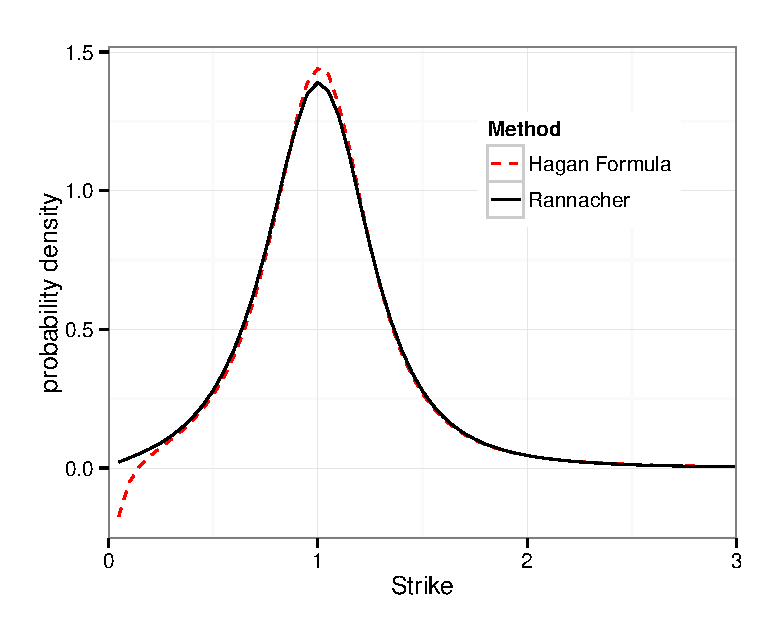
\includegraphics[width=7cm]{density_hagan_ran_500_5.eps}}
  \subfigure[Crank-Nicolson first 4 time steps with 5 time steps]{\label{fig:density_hagan_cn_500_5_5}
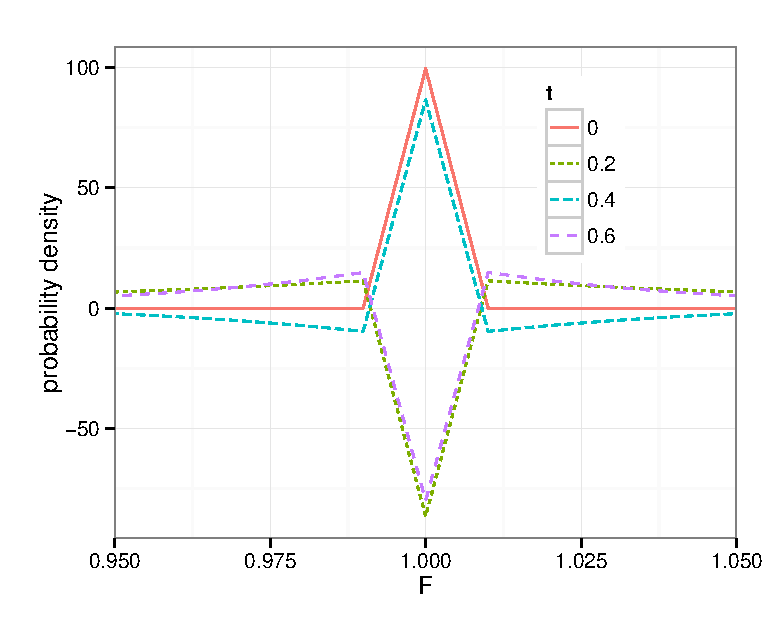
\includegraphics[width=7cm]{density_hagan_cn_500_5_5.eps}}
  \subfigure[Rannacher first 4 time steps with 5 time steps]{\label{fig:density_hagan_ran_500_5_5}
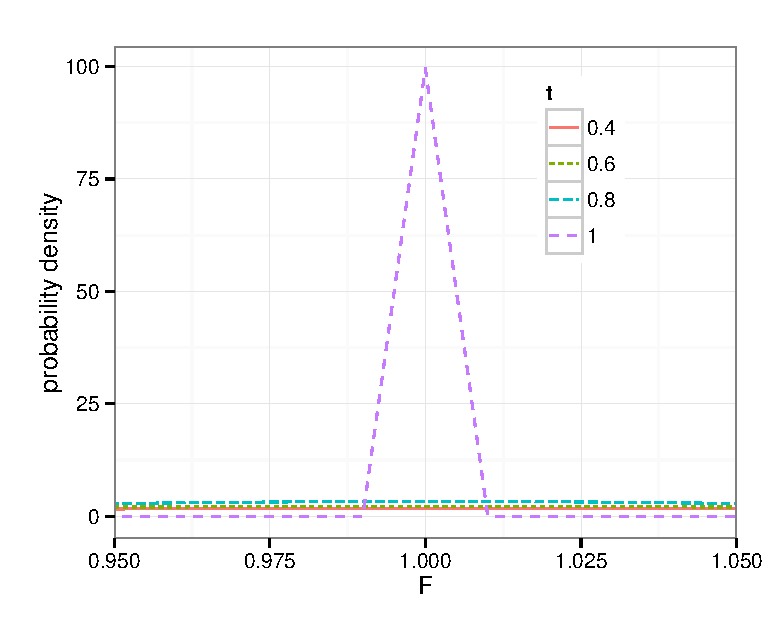
\includegraphics[width=7cm]{density_hagan_ran_500_5_5.eps}}
  \subfigure[LMG3 first 4 time steps with 5 time steps]{\label{fig:density_hagan_lmg3_500_5_5}
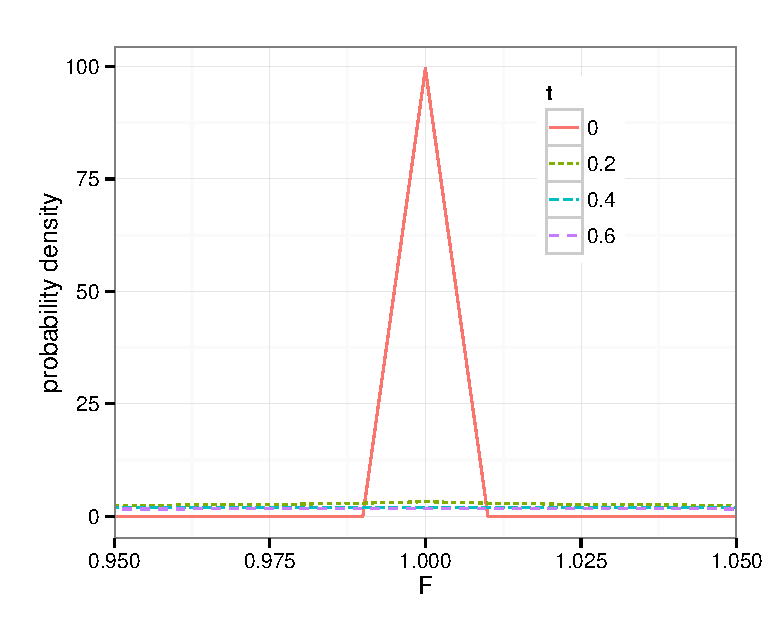
\includegraphics[width=7cm]{density_hagan_lmg3_500_5_5.eps}}
  \end{center}
     \caption{\label{fig:density_hagan_lmg2_500_10} Probability density in Hagan PDE using a total of 5 time-steps}
\end{figure}
With the same parameters as in section \ref{section_cn}, Figure \ref{fig:density_hagan_ran_500_5_0} shows a smooth positive probability density using only a total of 5 time-steps when Rannacher smoothing is applied to Crank-Nicolson. The density computed using second or third order Lawson-Morris-Gourlay (LMG2, LMG3), Lawson-Swayne (LS), TR-BDF2 or Richardson extrapolation on implicit Euler would look very similar. Figures \ref{fig:density_hagan_ran_500_5_5} and \ref{fig:density_hagan_lmg3_500_5_5} show no apparent oscillations in the first steps.
In contrast, Crank-Nicolson had strong oscillations visible at $t_N=T$ with 40 time steps.

\subsection{Performance}
\subsubsection{Hagan Example}
With the same parameters as in section \ref{section_cn}, we look at the maximum error in the probability density with a varying number of time-steps compared to a Crank-Nicolson scheme with 5120 points for the rate dimension and 81920 time-steps. 

\begin{figure}[htb]
  \begin{center}  
  \subfigure[Accuracy vs. number of time steps]{\label{fig:perf_hagan_500_steps}
  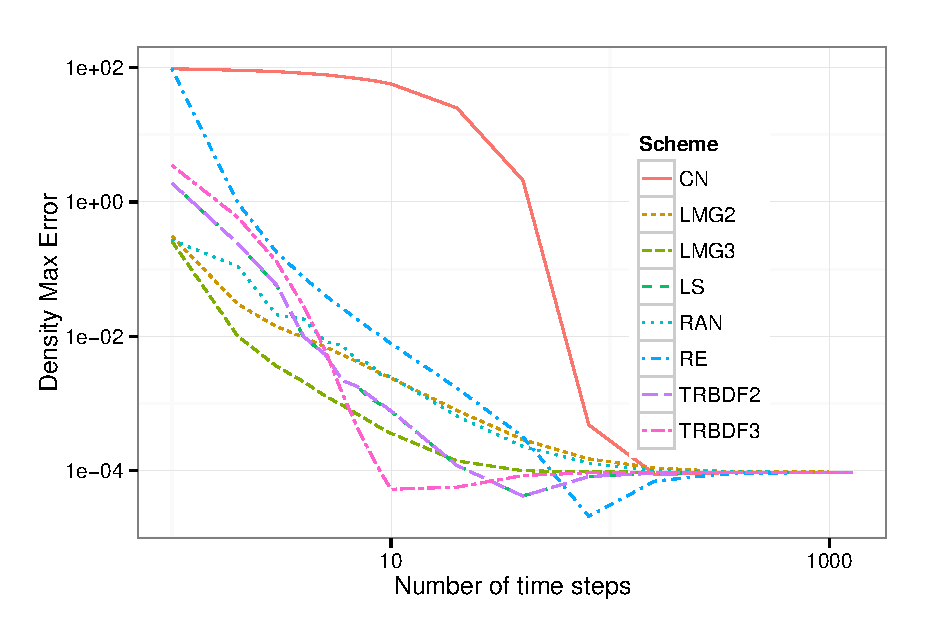
\includegraphics[width=7cm]{perf_density_hagan_500_steps.eps}}
  \subfigure[Accuracy vs. time]{
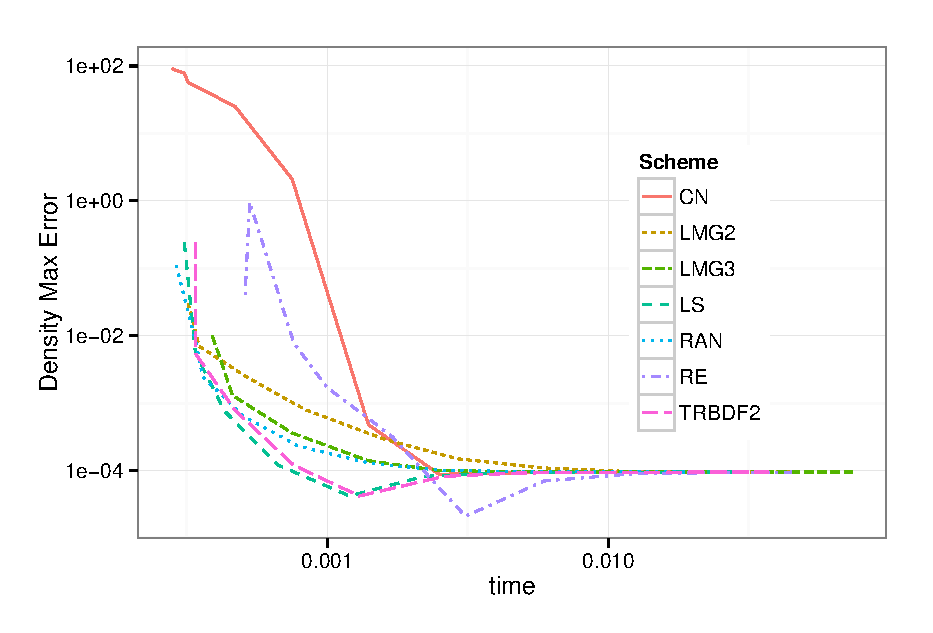
\includegraphics[width=7cm]{perf_density_hagan_500_time.eps}}
    \end{center}
     \caption{\label{fig:perf_hagan_500} Performance on Hagan example}
\end{figure}

%show convergence graph
Other tests we performed indicate that the implied volatility maximum error or even the at-the-money implied volatility error would lead to similar conclusions. Furthermore, a Black implied volatility with an absolute error under 0.1\% was achieved with only 2 time steps for LMG3, Lawson-Swayne and TR-BDF2, 5 time steps for LMG2, and 10 steps for RAN. Lawson-Swayne is the most efficient scheme on this problem, closely followed by TR-BDF2, Rannacher and LMG3.

\subsubsection{Andreasen-Huge Example}
We consider the SABR parameters used in \citep{andreasen2011zabr}: $\alpha=0.0873, \beta=0.7, \rho=-0.48, \nu=0.47$ with a forward of $f=0.025$ and a maturity $T=10.0$ and look at the maximum error in implied volatility between $0.2f$ and $2f$.

\begin{figure}[htb]
  \begin{center}  
  \subfigure[Accuracy vs. number of time steps]{\label{fig:perf_ah_500_steps}
  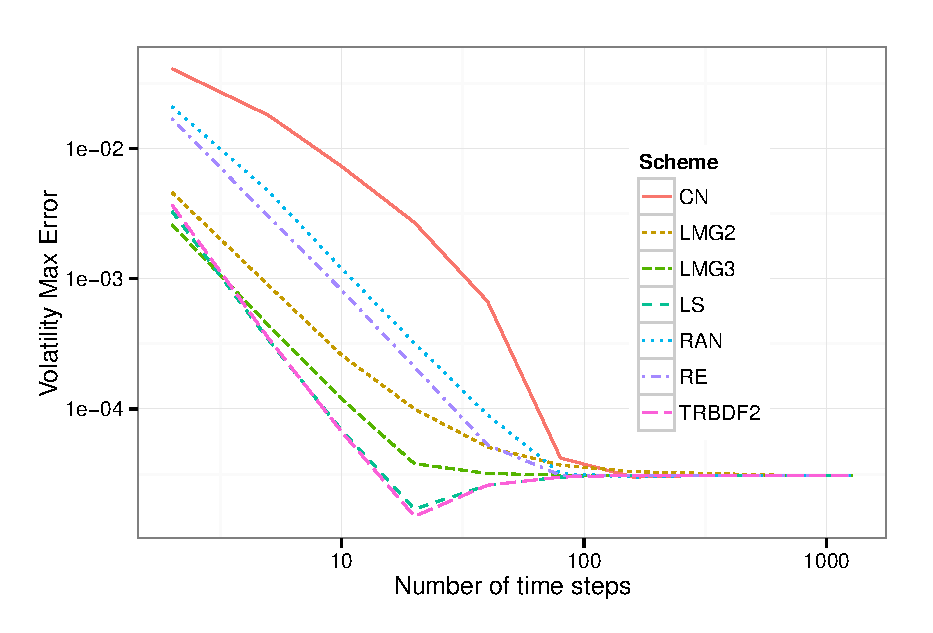
\includegraphics[width=7cm]{perf_vol_ah_500_steps.eps}}
  \subfigure[Accuracy vs. time]{
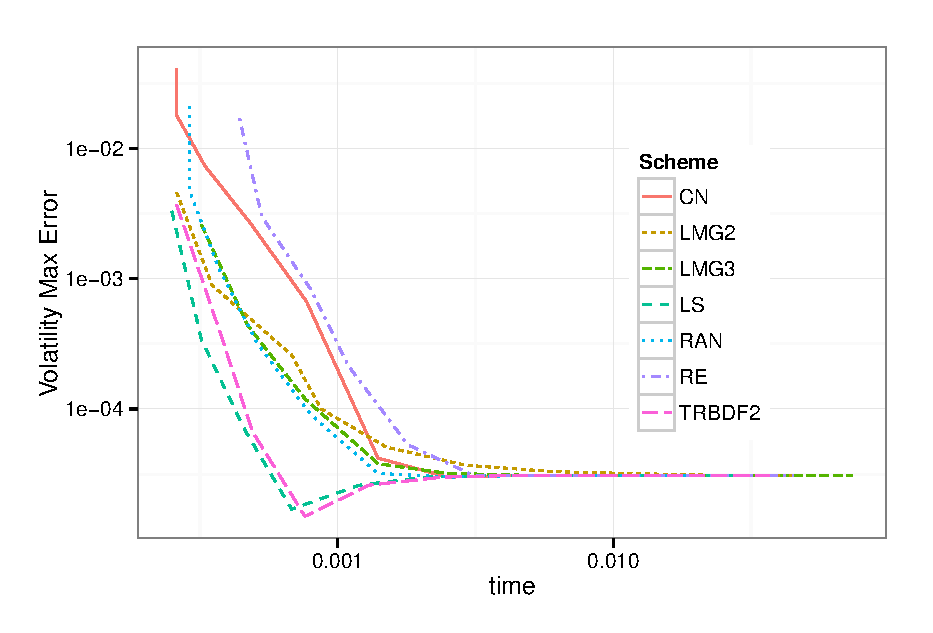
\includegraphics[width=7cm]{perf_vol_ah_500_time.eps}}
    \end{center}
     \caption{\label{fig:perf_ah_500} Performance on Andreasen-Huge example}
\end{figure}


%show convergence graph

Only 2 time-steps are enough with  LMG3 for good accuracy, and 5 for LMG2, LS, RAN and TR-BDF2. 
\section{Conclusion}
It is possible to accurately compute option prices under the arbitrage free SABR approach with very few time-steps, even for long maturities. The Rannacher smoothing is a particularly simple and efficient way to improve accuracy significantly compared to Crank-Nicolson on this problem. Depending on the SABR parameters, other schemes, like TR-BDF2 or Lawson-Swayne can be even more efficient.
This makes \citep{hagan2013arbitrage} particularly competitive to the one step finite difference approach of \citep{andreasen2011zabr}.
\bibliographystyle{rAMF}
%\bibliographystyle{ieeetr}
\bibliography{lefloch_sabr_fdm}
\newpage
\appendix
\section{Moment conservation in Implicit Euler}
We have for implicit Euler:

\begin{eqnarray}
Q_j^{n+1} - \frac{\delta}{h^2}\left(M_{j+1}^{n+1}Q_{j+1}^{n+1}-2M_j^{n+1}Q_j^{n+1}+M_{j-1}^{n+1}Q_{j-1}^{n+1}\right) = Q_j^n \\
Q_L^{n+1}-Q_L^n = \frac{\delta}{h}\left(M_1^{n+1}Q_1^{n+1}-M_0^{n+1}Q_0^{n+1}\right)\\
Q_R^{n+1}-Q_R^n = \frac{\delta}{h}\left(M_{J+1}^{n+1}Q_{J+1}^{n+1}-M_{J}^{n+1}Q_J^{n+1}\right)
\end{eqnarray}

with absorbing boundary conditions
$$M_0^{n+1}Q_0^{n+1} + M_1^{n+1}Q_1^{n+1} = 0 $$
$$M_{J+1}^{n+1}Q_{J+1}^{n+1} + M_J^{n+1}Q_J^{n+1} = 0 $$

Summing over $j$ yields:
\begin{align}
\sum_{j=1}^{J} h (Q_j^{n+1}-Q_j^n) &= \frac{\delta}{h}\left(M_{J+1}^{n+1}Q_{J+1}^{n+1}-M_J^{n+1}Q_J^{n+1}-M_1^{n+1}Q_1^{n+1}+M_0^{n+1}Q_0^{n+1}\right)\\
&= -(Q_L^{n+1}-Q_L^n)+(Q_R^{n+1}-Q_R^n)
\end{align}

The total probability follows:
\begin{align}
Q_L^{n+1}+\sum_{j=1}^J hQ_j^{n+1} + Q_R^{n+1} &= Q_L^{n}+\sum_{j=1}^J hQ_j^{n} + Q_R^{n} 
\end{align}
The total probability is conserved from one time-step to another.

Let's look now at the conservation of the forward. We multiply equation by $F_j$ and sum, using the fact that the forward obeys $F_{j+1}-2F_{j}+F_{j-1}=0$:
\begin{eqnarray}
\sum_{j=1}^{J} h F_j (Q_j^{n+1}-Q_j^n) = \\ \frac{\delta}{h}\left(F_J M_{J+1}^{n+1}Q_{J+1}^{n+1}-F_{J+1}M_J^{n+1}Q_J^{n+1}-F_0 M_1^{n+1}Q_1^{n+1}+F_1 M_0^{n+1}Q_0^{n+1}\right)\\
F_{min}(Q_L^{n+1}-Q_L^n)+ \sum_{j=1}^{J} h F_j (Q_j^{n+1}-Q_j^n) +F_{max}(Q_R^{n+1}-Q_R^n) = \\ \frac{\delta}{2}\left(M_{1}^{n+1}Q_{1}^{n+1}+M_0^{n+1}Q_0^{n+1}\right)-\frac{\delta}{2}\left(M_{J+1}^{n+1}Q_{J+1}^{n+1}+M_J^{n+1}Q_J^{n+1}\right)
\end{eqnarray}
The boundary conditions ensures that the right hand side is 0, and therefore the forward is conserved between time-steps.
 
\section{Moment conservation in TR-BDF2}
As the first stage is just Crank-Nicolson applied to a fraction of time-step, \citep{hagan2013arbitrage} already proved the first stage is moment preserving. We will now prove that the BDF2 stage is also moment preserving. We use $n+\alpha$ to represent the value at $t_{n}+\alpha \delta$. We have for the second stage:

$$(2-\alpha)Q_j^{n+1}-\frac{1}{\alpha}Q_j^{n+\alpha}+\frac{(1-\alpha)^2}{\alpha}Q_j^n=\delta(1-\alpha)\frac{\partial^2}{\partial F^2}M^{n+1}Q^{n+1}$$ 

$$= (1-\alpha)\frac{\delta}{h^2}\left(M_{j+1}^{n+1}Q_{j+1}^{n+1}-2M_{j}^{n+1}Q_{j}^{n+1}+M_{j-1}^{n+1}Q_{j-1}^{n+1}\right)$$

with absorbing boundary conditions
$$M_0^{n+1}Q_0^{n+1} + M_1^{n+1}Q_1^{n+1} = 0 $$
$$M_{J+1}^{n+1}Q_{J+1}^{n+1} + M_J^{n+1}Q_J^{n+1} = 0 $$

After $Q_j^{n+1}$ is updated, one can update $Q_L^{n+1}$ and $Q_R^{n+1}$

$$(2-\alpha)Q_L^{n+1}-\frac{1}{\alpha}Q_L^{n+\alpha}+\frac{(1-\alpha)^2}{\alpha}Q_L^n=(1-\alpha)\frac{\delta}{h}\left(M_1^{n+1}Q_1^{n+1} - M_0^{n+1}Q_0^{n+1}\right)$$

$$(2-\alpha)Q_R^{n+1}-\frac{1}{\alpha}Q_R^{n+\alpha}+\frac{(1-\alpha)^2}{\alpha}Q_R^n=-(1-\alpha)\frac{\delta}{h}\left(M_{J+1}^{n+1}Q_{J+1}^{n+1} - M_J^{n+1}Q_J^{n+1}\right)$$

Let's look at the total probability conservation:
\begin{eqnarray}
& &h\sum_{j=1}^J \left[(2-\alpha)Q_j^{n+1}-\frac{1}{\alpha}Q_j^{n+\alpha}+\frac{(1-\alpha)^2}{\alpha}Q_j^n\right]\\
&=& (1-\alpha)\frac{\delta}{h}\left(M_{J+1}^{n}Q_{J+1}^{n}-M_{J}^{n}Q_{J}^{n}-
M_{1}^{n}Q_{1}^{n}+M_{0}^{n}Q_{0}^{n}\right)\\
&=&-\left[(2-\alpha)Q_L^{n+1}-\frac{1}{\alpha}Q_L^{n+\alpha}+\frac{(1-\alpha)^2}{\alpha}Q_L^n\right]\\
& &-\left[(2-\alpha)Q_R^{n+1}-\frac{1}{\alpha}Q_R^{n+\alpha}+\frac{(1-\alpha)^2}{\alpha}Q_R^n\right]
\end{eqnarray}

in which case, since we already confirmed that total probability was preserved at $Q^{n+\alpha}$, we can see that the BDF2 stage will also preserve total probability to $Q^n$.

\begin{eqnarray}
& &(2-\alpha)\left[Q_L^{n+1} + h\sum_{j=1}^J Q_j^{n+1} +Q_R^{n+1}\right]\\
&=&\frac{1}{\alpha}\left[Q_L^{n+\alpha} + h\sum_{j=1}^J Q_j^{n+\alpha} +Q_R^{n+\alpha}\right]\\
& &-\frac{(1-\alpha)^2}{\alpha}\left[Q_L^{n} + h\sum_{j=1}^J Q_j^{n} +Q_R^{n}\right]\\
&=& (2-\alpha)
\end{eqnarray}

Now recall that our grid has even spacing, and so $F_{j+1}-2F_j+F_j=0$, then

\begin{eqnarray}
& &h\sum_{j=1}^J F_j\left[(2-\alpha)Q_j^{n+1}-\frac{1}{\alpha}Q_j^{n+\alpha}+\frac{(1-\alpha)^2}{\alpha}Q_j^n\right]\\
&=&(1-\alpha)\frac{\delta}{h}\left(F_JM_{J+1}^{n+1}Q_{J+1}^{n+1}-F_{J+1}M_J^{n+1}Q_J^{n+1}\right)\\
& &+ (1-\alpha)\frac{\delta}{h}\left(F_1M_{0}^{n+1}Q_{0}^{n+1}-F_{0}M_1^{n+1}Q_1^{n+1}\right)
\end{eqnarray}

then, recalling that $F_{min}=\frac{1}{2}(F_0+F_1)$ and $F_{max}=\frac{1}{2}(F_J+F_{J+1})$ and $F_1-F_0=F_{J+1}-F_{J}=h$, 

\begin{eqnarray}
& &F_{min}\left[(2-\alpha)Q_L^{n+1}-\frac{1}{\alpha}Q_L^{n+\alpha}+\frac{(1-\alpha)^2}{\alpha}Q_L^n\right]\\
&+& h\sum_{j=1}^J F_j\left[(2-\alpha)Q_j^{n+1}-\frac{1}{\alpha}Q_j^{n+\alpha}+\frac{(1-\alpha)^2}{\alpha}Q_j^n\right]\\
&+&F_{max}\left[(2-\alpha)Q_R^{n+1}-\frac{1}{\alpha}Q_R^{n+\alpha}+\frac{(1-\alpha)^2}{\alpha}Q_R^n\right]\\
&=&(1-\alpha)\frac{\delta}{2}\left(M^{n+1}_1Q_1^{n+1}+M_0^{n+1}Q_0^{n+1}\right)\\
& &+(1-\alpha)\frac{\delta}{2}\left(M^{n+1}_{J+1}Q_{J+1}^{n+1}+M_J^{n+1}Q_J^{n+1}\right)\\
&=&0
\end{eqnarray}
Collecting terms, we see that

$$(2-\alpha)\left[F_{min}Q_L^{n+1} + h\sum_{j=1}^J F_jQ_j^{n+1} +F_{max}Q_R^{n+1}\right]=\frac{1}{\alpha}f - \frac{(1-\alpha)^2}{\alpha}f$$
and so the forward is preserved by BDF2 at $t_{n+1}$.

Checking the moments is very useful way to check the implementation in code.

\section{Sample Numbers}
\begin{table}[h]
\begin{center}
\begin{tabular}{|c|r|r|r|r|}
\hline
Scheme & h & Q(f) & QL & QR\\ \hline
LMG3 & 0.010050251256 & 1.385108845032 & 0.036878097804 & 0.000775853690\\
LS & 0.010050251256 & 1.378405046490 & 0.036466946406 & 0.000797983056\\
LMG2 & 0.010050251256 & 1.390737156096 & 0.037351038244 & 0.000808345304\\
RE & 0.010050251256 & 1.342391047522 & 0.036966009503 & 0.000850746756\\
TRBDF2 & 0.010050251256 & 1.378368965895 & 0.036464938933 & 0.000797736766\\
CN & 0.010050251256 & -76.222597308083 & 0.036145997780 & 0.000811969902\\
\hline
\end{tabular}
\caption{Sample values using 500 points and 5 time-steps, $\alpha=35\%, \beta=0.25, \rho=-10\%, \nu=100\%, T=1, f=1, F_{max}=5, \delta=0.2$}
\end{center}
\end{table} 

\section{Performance Table}
\begin{table}[h]
\begin{center}
\begin{tiny}
\begin{tabular}{|l|l|c|r|r||l|l|c|r|r|}
\hline
SpaceSteps & TimeSteps & Scheme & MaxError & Time & SpaceSteps & TimeSteps & Scheme & MaxError & Time\\ \hline
500 & 2 & CN & 9.1e+01 & 2.5e-04&      500 & 80 & CN & 4.8e-04 & 1.4e-03\\
500 & 2 & RAN & 1.1e-01 & 3.0e-04&     500 & 80 & RAN & 1.3e-04 & 1.4e-03\\
500 & 2 & LMG2 & 3.0e-02 & 2.8e-04&    500 & 80 & LMG2 & 1.5e-04 & 2.9e-03\\
500 & 2 & LMG3 & 1.0e-02 & 3.3e-04&    500 & 80 & LMG3 & 9.6e-05 & 4.7e-03\\
500 & 2 & LS & 2.4e-01 & 2.7e-04&      500 & 80 & LS & 8.2e-05 & 2.1e-03\\
500 & 2 & TRBDF2 & 2.4e-01 & 2.8e-04&  500 & 80 & TRBDF2 & 8.2e-05 & 2.5e-03\\
500 & 2 & RE & 9.6e-01 & 4.7e-04&      500 & 80 & RE & 2.1e-05 & 3.1e-03\\
500 & 5 & CN & 7.8e+01 & 3.0e-04&      500 & 160 & CN & 8.8e-05 & 2.5e-03\\
500 & 5 & RAN & 8.3e-03 & 3.3e-04&     500 & 160 & RAN & 1.0e-04 & 2.6e-03\\
500 & 5 & LMG2 & 7.0e-03 & 4.0e-04&    500 & 160 & LMG2 & 1.1e-04 & 5.6e-03\\
500 & 5 & LMG3 & 1.3e-03 & 5.3e-04&    500 & 160 & LMG3 & 9.5e-05 & 9.3e-03\\
500 & 5 & LS & 5.4e-03 & 3.5e-04&      500 & 160 & LS & 9.2e-05 & 4.1e-03\\
500 & 5 & TRBDF2 & 5.4e-03 & 3.8e-04&  500 & 160 & TRBDF2 & 9.2e-05 & 4.7e-03\\
500 & 5 & RE & 4.1e-02 & 5.9e-04&      500 & 160 & RE & 7.0e-05 & 5.9e-03\\
500 & 10 & CN & 5.7e+01 & 3.7e-04&     500 & 320 & CN & 9.3e-05 & 4.9e-03\\
500 & 10 & RAN & 2.5e-03 & 4.1e-04&    500 & 320 & RAN & 9.7e-05 & 4.9e-03\\
500 & 10 & LMG2 & 2.4e-03 & 5.2e-04&   500 & 320 & LMG2 & 9.8e-05 & 1.2e-02\\
500 & 10 & LMG3 & 3.6e-04 & 7.4e-04&   500 & 320 & LMG3 & 9.5e-05 & 1.9e-02\\
500 & 10 & LS & 7.7e-04 & 4.5e-04&     500 & 320 & LS & 9.4e-05 & 7.9e-03\\
500 & 10 & TRBDF2 & 7.7e-04 & 4.7e-04& 500 & 320 & TRBDF2 & 9.4e-05 & 9.2e-03\\
500 & 10 & RE & 7.8e-03 & 6.8e-04&     500 & 320 & RE & 8.9e-05 & 1.2e-02\\
500 & 20 & CN & 2.5e+01 & 5.5e-04&     500 & 640 & CN & 9.5e-05 & 9.6e-03\\
500 & 20 & RAN & 6.5e-04 & 5.1e-04&    500 & 640 & RAN & 9.5e-05 & 9.6e-03\\
500 & 20 & LMG2 & 7.9e-04 & 8.9e-04&   500 & 640 & LMG2 & 9.6e-05 & 2.2e-02\\
500 & 20 & LMG3 & 1.4e-04 & 1.3e-03&   500 & 640 & LMG3 & 9.5e-05 & 3.7e-02\\
500 & 20 & LS & 1.2e-04 & 6.7e-04&     500 & 640 & LS & 9.5e-05 & 1.6e-02\\
500 & 20 & TRBDF2 & 1.2e-04 & 7.5e-04& 500 & 640 & TRBDF2 & 9.5e-05 & 1.8e-02\\
500 & 20 & RE & 1.7e-03 & 1.0e-03&     500 & 640 & RE & 9.3e-05 & 2.3e-02\\
500 & 40 & CN & 2.1e+00 & 7.6e-04&     500 & 1280 & CN & 9.5e-05 & 1.9e-02\\
500 & 40 & RAN & 2.3e-04 & 9.0e-04&    500 & 1280 & RAN & 9.5e-05 & 1.9e-02\\
500 & 40 & LMG2 & 2.9e-04 & 1.8e-03&   500 & 1280 & LMG2 & 9.5e-05 & 4.4e-02\\
500 & 40 & LMG3 & 1.0e-04 & 2.5e-03&   500 & 1280 & LMG3 & 9.5e-05 & 7.3e-02\\
500 & 40 & LS & 4.2e-05 & 1.2e-03&     500 & 1280 & LS & 9.5e-05 & 3.1e-02\\
500 & 40 & TRBDF2 & 4.2e-05 & 1.4e-03& 500 & 1280 & TRBDF2 & 9.5e-05 & 3.7e-02\\
500 & 40 & RE & 3.2e-04 & 1.7e-03&     500 & 1280 & RE & 9.5e-05 & 4.5e-02\\\hline

\end{tabular}
\end{tiny}
\caption{Density and time taken for various finite difference schemes with $\alpha=35\%, \beta=0.25, \rho=-10\%, \nu=100\%, T=1, f=1, F_{max}=5$}
\end{center}
\end{table} 

\end{document}
